\subsubsection{Extending to Quantum Mechanics}
\begin{wrapfigure}{r}{0.4\textwidth}%
	% \centering%
	\begin{center}
		% 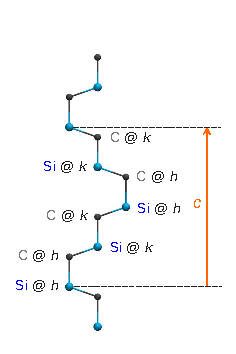
\includegraphics[width=0.38\textwidth]{figures/SiC-non-equiv-sites.pdf}%
		% MAGNETIC MOMENT ATOM
\begin{tikzpicture}[thick, scale=1.5]
  \def\rn{0.3}
  \def\re{0.15}
  \def\Rx{1.5}
  \def\Ry{0.5}
  %\draw[dashed] (-100:1.5*\rn) -- (80:1.5*\rn);
  \draw[dashed] (-\Rx,0) arc (180:0:{\Rx} and {\Ry});
  \draw[mu vector] (0,-1.8*\rn) -- (0,2.9*\rn) node[right] {$\vb*{\mu}$};
  \draw[charge+] (0,0) circle (\rn) node[scale=1.4] {+};
  \draw[dashed] (\Rx,0) arc (0:-180:{\Rx} and {\Ry});
  \draw[charge-]
    (-40:{\Rx} and {\Ry}) circle (\re) node[scale=0.8] {$-$}
    node[below right=0.2] {e};
  \draw[->]
    (-55:{1.15*\Rx} and {1.2*\Ry}) arc (-55:-72:{1.15*\Rx} and {1.2*\Ry});
  \draw[current]
    (-140:{1.15*\Rx} and {1.2*\Ry}) arc (-140:-100:{1.15*\Rx} and {1.2*\Ry})
    node[midway,below] {$I$};
\end{tikzpicture}

		\caption{Schematic of electron in orbit generating a magnetic moment.}%
	\end{center}
\end{wrapfigure}%
Since the gyromagnetic ratio was calculated considering the motion of dipole in a loop, we may extend this to an electron in an orbit.
The fundamental change required to extend the model to quantum mechanics is the treatment of angular momentum which should now be quantised.
Thus, we replace our classical approximation of $\vec{G} = \vec{r} \times \vec{p}$ with the equation for the eigenvalues of the quantum mechanical representation of orbital angular momentum,
\begin{equation}
	\hat{G} = \hbar \hat{L}
	\label{eq:orbital_angular_momentum}
\end{equation}
where $\hat{L}$ is the operator of the orbital angular momentum (quantum number of orbital momentum).
The angular momentum and total energy are conserved in general in a closed system.

We consider the time independent \index{Shr\"odinger equation}{Shr\"odinger equation}
\begin{equation}
	\hat{H} \Psi_n = E_n \Psi_n
	\label{eq:TISE}
\end{equation}

and choose $\Psi_n$ such that it is an eigenfunction of the Hamiltonian, the total angular momentum squared ($L^2 = L_x^2 + L_y^2 + L_z^2$) and exactly one directional component of the angular momentum which is by convention chosen as $L_z$.

According to quantum mechanics the projection of $L$ along the \index{quantisation axis} ($m_L$) may take integer values $-L, -L + 1, \dots, L-1, L$.
Thus, we may describe a given quantum state by the angular momentum $L$ and it's projection $m_L$. Thus, using \index{Dirac notation}{Dirac Notation} we write
\begin{eqnarray}
	&\hat{H}\ket{L, m_L} &= E\ket{L, m_L} \\
	&\hat{L}^2\ket{L, m_L} &= L(L+1)\ket{L, M_L} \\
	&\hat{L}_z\ket{L, m_L} &= m_L\ket{L, m_L}. \label{eq:zthcomponent}
\end{eqnarray}
Thus, the operator which describes the orbital magnetic moment may be written using  \eqref{eq:gyromagnetic_ratio_electrons}, \eqref{eq:orbital_angular_momentum} as
\begin{equation}
	\hat{\vec{\mu}}_L = \gamma \hat{\vec{G}}_L = \gamma \hbar \hat{\vec{L}} = \frac{e\hbar}{2m_e c}\hat{\vec{L}}.
	\label{eq:orbital_magnetic_moment_operator}
\end{equation}

This leads to a quantity known as the \textbf{\index{Bohr magneton}{Bohr Magneton}}, $\mu_B$, given by \cite{Ramamurti1995-wg}
\begin{equation}
	\mu_B = \frac{|e|\hbar}{2m_e c}.
	\label{eq:bohr_magneton}
\end{equation}

Using this we may write \eqref{eq:orbital_magnetic_moment_operator} as
\begin{equation}
	\hat{\vec{\mu}}_L = -\mu_B\hat{\vec{L}}.
	\label{eq:orbital_magnetic_moment_operator_bohr_magneton}
\end{equation}


\subsection{g-factor}
The above expression is valid for the orbital electron but may be extended to a more general system by introducing a \index{g-factor}{g-factor}. The g-factor is equivalent to a dimensionless gyromagnetic ratio \cite{giancoli2008physics}, so \eqref{eq:orbital_magnetic_moment_operator_bohr_magneton} may be written with $g=1$ as
\begin{equation}
	\hat{\vec{\mu}}_L = -g\mu_B\hat{ \vec{L}}.
	\label{eq:orbital_magnetic_moment_operator_bohr_magneton_g_factor}
\end{equation}


